\documentclass{../../oss-apphys-exam}

\begin{document}
%\genheader

\gentitle{13}{ROTATIONAL MOTION}

%\begin{center}
%  \fcolorbox{black}{pink!30}{
%    \begin{minipage}{\linewidth}
%      \large\textbf{Please note that We will \emph{not} have enough time to
%        review every homework question in class. Instead, multiple-choice
%        questions are taken up in a pre-recorded video. Please follow the link
%        posted on Classkick to review the questions. The video is not long, but
%        is well worth your time if you want to learn. Ths homework set is due
%        at the end of Class 17 as usual.}
%    \end{minipage}
%  }
%\end{center}

\begin{questions}
  \classkickMCinstructions
  
  \question What defines a moment arm?
  \begin{choices}
    \choice The distance parallel to the line of action of the force
    \choice The distance parallel to the line of action of the force from the
    pivot point
    \choice The length of the lever
    \choice The perpendicular distance from the pivot to the line of action of
    the force
    \choice $F = |F|cos(\theta)x$
  \end{choices}

  \question When a figure skater performs a spin on ice with her arms
  outstretched, what happens when she brings her arms close to her body?
  \begin{choices}
    \choice Her angular acceleration decreases because her moment of inertia
    was decreased.
    \choice Her angular acceleration increases because her moment of inertia
    was decreased.
    \choice Her angular velocity decreases because her moment of inertia was
    decreased.
    \choice Her angular velocity increases because her moment of inertia was
    decreased.
    \choice Her angular displacement increases because her moment of inertia
    was decreased
  \end{choices}

\question A metre stick of mass \SI{.1}{\kilo\gram} rests on a table as
  shown. A length of \SI{40}{\centi\metre} extends over the edge of the table.
  How far from the edge of the table could a \SI{.05}{\kilo\gram} mass be
  placed on the metre stick so that the stick just begins to tip?
  \begin{center}
    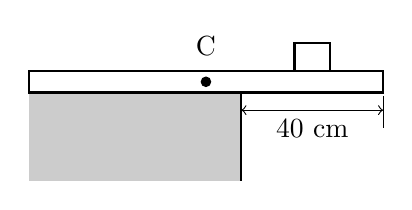
\begin{tikzpicture}[scale=4.5]
      \fill[gray!40] (0,-.25) rectangle (.6,0);
      \draw[thick] rectangle (1,.06);
      \draw[thick] (.6,0)--(.6,-.25);
      \draw[thick] (.75,.06) rectangle (.85,.14);
      \draw (1,-.01)--(1,-.1);
      \draw[<->] (.6,-.05)--(1,-.05) node[midway,below]{40 cm};
      \fill (.5,.03) circle(.015);
      \node at (.5,.13){C};
    \end{tikzpicture}
  \end{center}
  \begin{choices}
    \choice\SI5{\centi\metre}
    \choice\SI{10}{\centi\metre}
    \choice\SI{15}{\centi\metre}
    \choice\SI{20}{\centi\metre}
    \choice\SI{30}{\centi\metre}
  \end{choices}

  %\question A metre stick is balanced on a fulcrum at its centre, as shown. A
  %mass of \SI{5}{\kilo\gram} is hung on the left end of the stick, and a mass 
  %of \SI{2}{\kilo\gram} is hung on the right end. In order to balance the
  %system, a mass $m$ is hung at the 25-cm mark on the right
  %side. What is the value of the mass $m$?
  %\begin{center}
  %  \begin{tikzpicture}[scale=1.7,thick]
  %    \draw(-2,-.08) rectangle (2,.08);
  %    \fill circle (.035);
  %    \draw (-2,0)--(-2,-.5);
  %    \draw (2,0)--(2,-.6);
  %    \draw (-2.2,-.5) rectangle (-1.8,-1) node[midway]{\footnotesize 5 kg};
  %    \draw (2.2,-.6) rectangle (1.8,-.9) node[midway]{\footnotesize 2 kg};
  %    \draw (1,0) circle(.035);
  %    \draw (1,-.035)--(1,-.3);
  %    \draw (.9,-.3) rectangle (1.1,-.5) node[midway]{\footnotesize$m$};
  %    \fill[gray!50] (-.3,-.6) rectangle (.3,-.5);
  %    \draw (0,0)--(-.15,-.5)--(.15,-.5)--cycle;
  %    \draw (-.3,-.5)--(.3,-.5);
  %  \end{tikzpicture}
  %\end{center}
  %\begin{oneparchoices}
  %  \choice\SI{12}{\kilo\gram}
  %  \choice\SI6{\kilo\gram}
  %  \choice\SI4{\kilo\gram}
  %  \choice\SI3{\kilo\gram}
  %  \choice\SI2{\kilo\gram}
  %\end{oneparchoices}

 \uplevel{
    \textbf{Questions \ref{lightrod1}--\ref{lightrod2}}:
    A light rod of negligible mass is pivoted at point $P$ a distance $L$ from
    one end as shown. A mass $m$ is attached to the left end of the rod at
    a distance of $3L$ from the pivot, and another mass $4m$ is attached to the
    other end a distance $L$ from the pivot. The system begins from rest in the
    horizontal position.
    \begin{center}
      \begin{tikzpicture}[scale=1.5]
        \draw[very thick] (-3,0)--(1,0);
        \draw[thick] (1,-.2) rectangle (1.4,.2) node[midway]{$4m$};
        \draw[thick] (-3,-.11) rectangle (-3.22,.11) node[midway]{$m$};
        \fill circle(.05) node[above]{$P$};
        \node at (.5,.15){$L$};
        \node at (-1.5,.15){$3L$};
        \draw[vectors,rotate=40] (.35,0) arc (0:260:.35);
      \end{tikzpicture}
    \end{center}
  }


  \question The net torque acting on the system due to gravitational forces is
  \label{lightrod1}
  \begin{choices}
    \choice $4mgL$ clockwise
    \choice $3mgL$ clockwise
    \choice $3mgL$ counterclockwise
    \choice $mgL$ counterclockwise
    \choice $mgL$ clockwise
  \end{choices}
    
  \question The angular acceleration of the system when it is released from
  rest is
  \begin{choices}
    \choice zero
    \choice $\dfrac g{5L}$
    \choice $\dfrac g{4L}$
    \choice $\dfrac g{13L}$
    \choice $\dfrac gL$
  \end{choices}
  \label{lightrod2}
  
  \question A hoop of radius $R$ and mass $m$ has a rotational inertia of
  $mR^2$. The hoop rolls without slipping along a horizontal floor with a
  constant speed $v$ and then rolls up a long incline. The hoop can roll up the
  incline to a maximum vertical height of
  \begin{center}
    \begin{tikzpicture}
      \fill[gray!50] (0,-.2) rectangle(7,0);
      \draw[thick] (0,0)--(7,0);
      \draw[thick] (3.5,0)--(7,1.2)--(7,0);
      \draw[thick] (1.5,.4) circle (.4);
      \fill (1.5,.4) circle (.06);
      \draw[vectors] (1.5,.4)--(2.5,.4) node[right]{$v$};
      \draw[axes] (.95,.4) arc (180:45:.55);
      \draw[thick,<->] (7.2,0)--(7.2,1.2) node[midway,right]{$h$};
    \end{tikzpicture}
  \end{center}
  \begin{choices}
    \choice$\dfrac{v^2}{g}$
    \choice$\dfrac{2v^2}{g}$
    \choice$\dfrac{v^2}{2g}$
    \choice$\dfrac{4v^2}{g}$
    \choice$\dfrac{v^2}{4g}$
  \end{choices}

  %\question Two disks are fixed to a vertical axle that is rotating with a
  %constant angular speed $\omega$. The smaller disk has a mass $m$ and a radius
  %$r$, and the larger disk has a mass $2m$ and radius $2r$. The general equation
  %for the rotational inertia of a disk of mass $M$ and radius $R$ is
  %$\frac12MR^2$. The ratio of the angular momentum of the larger disk to
  %the smaller disk is
  %\begin{minipage}{.35\textwidth}
  %  \cpic{.7}{2disks}
  %\end{minipage}
  %\begin{minipage}{.3\textwidth}
  %  \begin{choices}
  %    \choice $1:4$
  %    \choice $4:1$
  %    \choice $1:2$
  %    \choice $2:1$
  %    \choice $8:1$
  %  \end{choices}
  %\end{minipage}
  
  \question Astronauts are conducting an experiment in a negligible gravity
  environment. Two spheres of mass $m$ are attached to either end of a light
  rod. As the rod and spheres float motionless in space, an astronaut launches
  a piece of sticky clay, also of mass $m$, toward one of the spheres so that
  the clay strikes and sticks to the sphere perpendicular to the rod. Which of
  the following statements is true of the motion of the rod, clay, and spheres
  after the collision?
  \begin{center}
    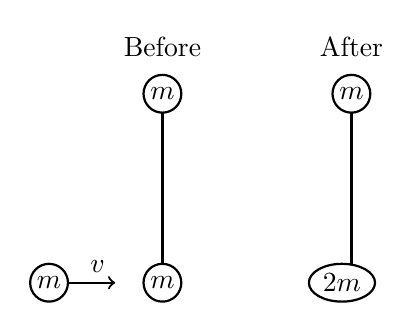
\begin{tikzpicture}[scale=1.2]
      \begin{scope}[thick]
        \draw circle (.2) node{$m$};
        \draw (0,2) circle (.2) node{$m$};
        \draw (0,.2)--(0,1.8);
        \draw (-1.2,0) circle (.2) node{$m$};
        \draw[->] (-1,0)--(-.5,0) node[above left]{$v$};
        
        \draw (1.9,0) ellipse (.35 and .2) node{$2m$};
        \draw (2,2) circle (.2) node{$m$};
        \draw (2,.2)--(2,1.8);
      \end{scope}
      \node at (0,2.5){Before};
      \node at (2,2.5){After};
    \end{tikzpicture}
  \end{center}
  \begin{choices}
    \choice Linear momentum is not conserved, but angular momentum is
    conserved.
    \choice Angular momentum is not conserved, but linear momentum is
    conserved.
    \choice Kinetic energy is conserved, but angular momentum is not
    conserved.
    \choice Kinetic energy is conserved, but linear momentum is not
    conserved.
    \choice Both linear momentum and angular momentum are conserved, but
    kinetic energy is not conserved.
  \end{choices}
  \newpage

  \uplevel{
    \centering
    \begin{tikzpicture}[thick]
      \draw (0.15,1)--+(0,-2);
      \fill[pattern=north east lines] (.15,-1) rectangle +(.2,2);
      \draw(.15,.18)--(0,.18) arc (90:270:.18)--(.15,-.18);
      \draw[fill=white] (0,.12) arc (90:-90:.12)--(-5,-.12)
      node[midway,below]{$L$} arc (270:90:.12) --(0,.12);
      \fill circle (.08) node[below=5]{$P$};
      \fill[white] circle (.04);
      \fill (-4.8,0) circle (.07);
      \draw (-4.8,0)-- +(0,2);
      \draw (-5.3,2)--+(1,0);
      \fill[pattern=north west lines] (-5.3,2) rectangle +(1,.2);
    \end{tikzpicture}
  }
  \question One end of a stick of length $L$, rotational inertia $I$, and mass
  $m$ is pivoted on an axle with negligible friction at point $P$, as shown
  above. The other end is tied to a string and held in a horizontal position.
  When the string is cut, the stick rotates counterclockwise. The angular speed
  $\omega$ of the stick when it reaches the bottom of its swing is
  \begin{choices}
    \choice$\dfrac{mgL}I$
    \choice$\sqrt{\dfrac{mgL}I}$
    \choice$\sqrt{\dfrac{2mgL}I}$
    \choice$\sqrt{\dfrac{mgL}{2I}}$
    \choice$\sqrt{\dfrac{4mgL}I}$
  \end{choices}
  
  \question A disk is mounted on a fixed axle. The rotational inertia of the
  disk is $I$. The angular velocity of the disk is decreased from $\omega_0$ to
  $\omega_f$ during a time $\Delta t$ due to friction in the axle. The
  magnitude of the average net torque acting on the wheel is
  \begin{choices}
    \choice $\dfrac{\omega_f-\omega_0}{\Delta t}$
    \choice $\dfrac{(\omega_f-\omega_o)^2}{\Delta t}$
    \choice $\dfrac{I(\omega_f-\omega_o)}{\Delta t}$
    \choice $\dfrac{I(\omega_f-\omega_o)^2}{\Delta t}$
    \choice $\dfrac{I(\omega_f-\omega_o)}{\Delta t^2}$
  \end{choices}
  
  \question The average power developed by the friction in the axle of the disk
  from the previous question to bring it to a complete stop is
  \begin{choices}
    \choice $\dfrac{\omega_0}{\Delta t}$
    \choice $\dfrac{(\omega_0)^2}{\Delta t}$
    \choice $\dfrac{I\omega_0}{2\Delta t}$
    \choice $\dfrac{I\omega_0^2}{2\Delta t}$
    \choice $\dfrac{I(\omega_f-\omega_0)}{\Delta t^2}$
  \end{choices}
  \newpage
  
  \question A rod of mass $M$, length $L$, and rotational inertia $I$ hangs
  at rest from a frictionless axle as shown. A ball of mass $m$ with a speed
  $v$ strikes the rod perpendicularly at the end of the rod. As a result
  of the collision, the ball stops. The angular speed of the rod immediately
  after the collision is
  \begin{center}
    \begin{tikzpicture}[thick]
      \draw[fill=lightgray] (-.15,.2) rectangle (.15,-3);
      \fill circle (.08);
      \draw (-1.7,-3) circle (.2) node{$m$};
      \draw[vectors] (-1.5,-3)--+(1,0) node[midway,above]{$\vec v$};
      \draw[|<->|] (-.4,.2)--(-.4,-3) node[midway,left]{$L$};
      \node[right] at (.3,-1.4) {$I$, $M$};
    \end{tikzpicture}
  \end{center}
  \begin{choices}
    \choice $vL$
    \choice $\dfrac vL$
    \choice $\dfrac{mv}I$
    \choice $\dfrac{mvL}I$
    \choice $\dfrac{mv}{IL}$
  \end{choices}
  
  \uplevel{
    \textbf{Questions \ref{hollow1}--\ref{hollow2}}: A hollow sphere of mass
    $m$ and radius $R$ begins from rest at a height $h$ and rolls down a rough
    inclined plane. The rotational inertia of the hollow sphere is
    $\dfrac23mR^2$.
    \begin{center}
      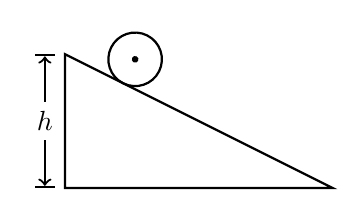
\begin{tikzpicture}[thick,scale=.85]
        \draw (0,0)--(-4,0)--(-4,2)--cycle;
        \draw[|<->|] (-4.3,2)--(-4.3,0) node[midway,fill=white]{$h$};
        \begin{scope}[rotate=-atan(2/4)]
          \draw (-3.5,.4) circle (.4);
          \fill (-3.5,.4) circle (.05);
        \end{scope}
      \end{tikzpicture}
    \end{center}
  }

  \question Which of the following diagrams best represents the forces acting
  on  the sphere as it rolls down the plane?

  \begin{oneparchoices}
    \choice
    \begin{tikzpicture}[scale=.6]
      \draw circle (1);
      \fill circle (.1);
      \draw[vectors] (0,0)--(0,-2) node[below]{$F_g$};
      \draw[vectors,rotate=45] (-1,0)--(2,0) node[right]{$N$};
      \draw[vectors,rotate=45] (-1,0)--(-1,1.5) node[left]{$f$};
    \end{tikzpicture}

    \choice
    \begin{tikzpicture}[scale=.6]
      \draw circle (1);
      \fill circle (.1);
      \draw[vectors] (0,0)--(0,-2) node[below]{$F_g$};
      \draw[vectors] (0,0)--(0,2) node[above]{$N$};
      \draw[vectors,rotate=45] (-1,0)--(-1,1.5) node[left]{$f$};
    \end{tikzpicture}

    \choice
    \begin{tikzpicture}[scale=.6]
      \draw circle (1);
      \fill circle (.1);
      \draw[vectors] (0,0)--(0,-2) node[below]{$F_g$};
      \draw[vectors,rotate=45] (-1,0)--(2,0) node[right]{$N$};
      \draw[vectors,rotate=45] (-1,0)--(-1,-1.5) node[right]{$f$};
    \end{tikzpicture}

    \choice
    \begin{tikzpicture}[scale=.6]
      \draw circle (1);
      \fill circle (.1);
      \draw[vectors] (0,0)--(0,-2) node[below]{$F_g$};
      \draw[vectors,rotate=45] (-1,0)--(2,0) node[right]{$N$};
      \draw[vectors] (-1,0)--(-1,1.5) node[above]{$f$};
    \end{tikzpicture}
      
    \choice
    \begin{tikzpicture}[scale=.6]
      \draw circle (1);
      \fill circle (.1);
      \draw[vectors,rotate=45] (0,0)--(0,-2) node[below]{$F_g$};
      \draw[vectors,rotate=45] (0,0)--(2,0) node[right]{$N$};
      \draw[vectors,rotate=45] (-1,0)--(-1,1.5) node[above]{$f$};
    \end{tikzpicture}
  \end{oneparchoices}
  \label{hollow1}
  
  \question The speed of the sphere when it reaches the bottom of the plane is
  \begin{choices}
    \choice $\sqrt{\dfrac{8gh}5}$
    \choice $\sqrt{\dfrac{6gh}5}$
    \choice $\sqrt{\dfrac{5gh}6}$
    \choice $\sqrt{\dfrac{7gh}{10}}$
    \choice $\sqrt{\dfrac{gh}2}$
  \end{choices}
  \label{hollow2}
  
  %\question A cylinder has a moment of inertia, $I$. How much time does it take
  %a torque, $\tau$, to increase its angular speed from $\omega_1$ to
  %$\omega_2$?
  %\begin{choices}
  %  \choice $\dfrac{I(\omega_2-\omega_1)}{\tau}$
  %  \choice $\dfrac{\tau}{I(\omega_2-\omega_1)}$
  %  \choice $I(\omega_2-\omega_1)\tau$
  %  \choice $\dfrac{2\tau}{I(\omega_2^2-\omega_1^2)}$
  %  \choice $\dfrac12I(\omega_2^2-\omega_1^2)\tau$
  %\end{choices}
  \newpage
  
%  \classkickFRQinstructions

%  \uplevel{
%    \cpic{.35}{disk1}
%  }
%  \question The disk shown above spins about the axle at its centre. A student's
%  experiments reveal that, while the disk is spinning, friction between the
%  axle and the disk exerts a constant torque on the disk.
%  \begin{parts}
%    \part At time $t=0$ the disk has an initial counterclockwise (positive)
%    angular velocity $\omega_0$. The disk later comes to rest at time $t=t_1$.
%    \begin{subparts}
%      \subpart On the grid at left below, sketch a graph that could represent
%      the disk's angular velocity as a function of time $t$ from $t=0$ until the
%      disk comes to rest at time $t=t_1$.
%      
%      \subpart On the grid at right below, sketch the disk's angular
%      acceleration as a function of time $t$ from $t=0$ until the disk comes to
%      rest at time $t=t_1$.   
%    \end{subparts}
%
%    \uplevel{
%      \cpic{.9}{graph1}
%    }
%    
%    \part The magnitude of the frictional torque exerted on the disk is
%    $\tau_0$ . Derive an equation for the rotational inertia $I$ of the disk in
%    terms of $\tau_0$, $\omega_0$, $t_1$, and physical constants, as
%    appropriate.
%    \newpage
%    
%    \part In another experiment, the disk again has an initial positive angular
%    velocity $\omega_0$ at time $t=0$. At $t=\dfrac12t_1$, the student starts
%    dripping oil on the contact surface between the axle and the disk to reduce
%    the friction. As time passes, more and more oil reaches that contact
%    surface, reducing the friction even further.
%    \begin{subparts}
%      \subpart On the grid at left below, sketch a graph that could represent
%      the disk's angular velocity as a function of time from $t=0$ to $t=t_1$,
%      which is the time at which the disk came to rest in part (a).
%
%      \subpart On the grid at right below, sketch the disk's angular
%      acceleration as a function of time from $t=0$ to $t=t_1$.
%    \end{subparts}
%
%    \uplevel{
%      \cpic{.9}{graph2}
%    }
%    
%    \part The student is trying to mathematically model the magnitude $\tau$ of
%     the torque exerted by the axle on the disk when the oil is present at
%     times $t>\dfrac12t_1$. The student writes down the following two
%     equations, each of which includes a positive constant ($C_1$ or $C_2$)
%     with appropriate units.
%     \begin{enumerate}
%       \item $\tau=C_1\left(t-\dfrac12t_1\right)$ (for $t>\dfrac12 t_1$)
%       \item $\tau=\dfrac{C_2}{\left(t+\dfrac12t_1\right)}$ (for
%         $t>\dfrac12t_1$)
%     \end{enumerate}
%     Which equation better mathematically models this experiment? Briefly
%     explain why the equation you selected is plausible and why the other
%     equation is not plausible.
%
%     \vspace{.1in}
%     \underline{\hspace{.3in}}Equation (1)\hspace{.2in}
%     \underline{\hspace{.3in}}Equation (2)
%  \end{parts}
%  \newpage
  \uplevel{
    \centering
    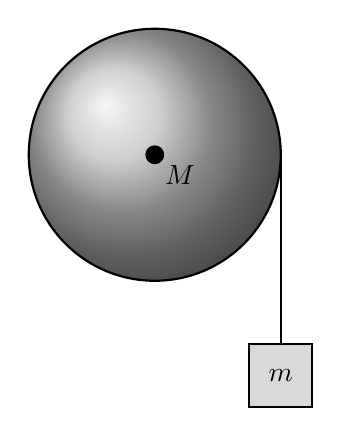
\begin{tikzpicture}[scale=.8,thick]
      \shade[ball color=lightgray] circle (2) node[below right]{$M$};
      \draw circle (2);
      \fill circle (.15);
      \draw (2,0)--(2,-3);
      \draw[fill=gray!30] (1.5,-3) rectangle +(1,-1) node[midway]{$m$};
    \end{tikzpicture}
  }
  \question A uniform sphere of mass $M$, and radius $R$ (rotational inertia
  $I=\dfrac25MR^2$) is free to rotate, without friction, about a horizontal axis
  through its centre. A string is wrapped around the sphere and is attached to
  a block of mass $m$ as shown in the figure above.
  \begin{parts}
    \part On the diagrams below, draw all forces (not components) that act on
    the sphere and the block. The forces should be drawn as arrows starting at
    where they are applied, and pointing away from the objects.
    \vspace{.75in}
    \begin{center}
      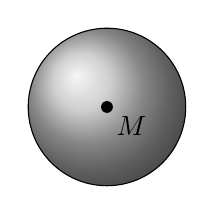
\begin{tikzpicture}[scale=.5]
        \shade[ball color=lightgray] circle (2) node[below right]{$M$};
        \draw circle (2);
        \fill circle (.15);
      \end{tikzpicture}
      \hspace{1.5in}
      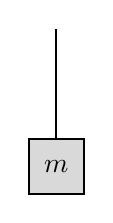
\begin{tikzpicture}[scale=.7,thick]
        \draw (2,-2)--(2,-4);
        \draw[fill=gray!30] (1.5,-4) rectangle (2.5,-5) node[midway]{$m$};
      \end{tikzpicture}
    \end{center}
    \vspace{.75in}
    \part Calculate the acceleration of the body.
    \vspace{\stretch1}
    \part Calculate the tension in the string.
    \vspace{\stretch1}
  \end{parts}
  \newpage

  \uplevel{
    \centering
    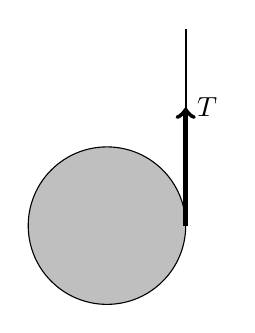
\begin{tikzpicture}[scale=.5]
      \draw[fill=lightgray] circle(2);
      \draw[thick] (2,0)--(2,5);
      \draw[ultra thick,->] (2,0)--(2,3) node[right]{$T$};
    \end{tikzpicture}
  }
  \question A uniform cylinder of mass $M$ and radius $R$ (rotational inertia
  $I=\frac12MR^2$) has a string wrapped around it. The string is held fixed,
  and the cylinder falls vertically as shown in the figure above. Find
  \begin{parts}
    \part the acceleration of the body, and
    \part the tension in the string.
  \end{parts}
  \newpage

  
%  % TAKEN FROM THE 2016 AP PHYSICS 1 EXAM FREE-RESPONSE QUESTION #1
%  \uplevel{
%    \cpic{.4}{wooden-wheel1}
%  }
%
%  \question A wooden wheel of mass $M$, consisting of a rim with spokes, rolls
%  down a ramp that makes an angle $\theta$ with the horizontal, as shown above.
%  The ramp exerts a force of static friction on the wheel so that the wheel
%  rolls without slipping.
%  \begin{parts}
%    \part On the diagram below, draw and label the forces (not components)
%    that act on the wheel as it rolls down the ramp, which is indicated by the
%    dashed line. To clearly indicate at which point on the wheel each force
%    is exerted, draw each force as a distinct arrow starting on, and pointing
%    away from, the point at which the force is exerted. The lengths of the
%    arrows need not indicate the relative magnitudes of the forces.
%
%    \vspace{.4in}
%    \cpic{.22}{wooden-wheel2}
%    \vspace{.4in}
%    
%    \part As the wheel rolls down the ramp, which force causes a change in
%    the angular velocity of the wheel with respect to its centre of mass?
%    Briefly explain your reasoning.
%    \vspace{\stretch1}
%
%    \part For this ramp angle, the force of friction exerted on the wheel is
%    less than the maximum possible static friction force. Instead, the
%    magnitude of the force of static friction exerted on the wheel is 40
%    percent of the magnitude of the force or force component directed opposite
%    to the force of friction. Derive an expression for the linear acceleration
%    of the wheel's centre of mass in terms of $M$, $\theta$, and physical
%    constants, as appropriate.
%    \vspace{\stretch1}
%    \newpage
%    
%    \uplevel{
%      In a second experiment on the same ramp, a block of ice, also with
%      mass $M$, is released from rest at the same instant the wheel is released
%      from rest, and from the same height. The block slides down the ramp with
%      negligible friction.
%    }
%    
%    \part Which object, if either, reaches the bottom of the ramp with the
%    greatest speed?
%
%    \vspace{.1in}
%    \underline{\hspace{.3in}} Wheel\hspace{.2in}
%    \underline{\hspace{.3in}} Block\hspace{.2in}
%    \underline{\hspace{.3in}} Neither; both reach the bottom with the same
%    speed.
%
%    \vspace{.1in}Briefly explain your answer, reasoning in terms of forces.
%    \vspace{\stretch1}
%      
%    \part Briefly explain your answer again, now reasoning in terms of
%    energy.
%    \vspace{\stretch3}
%  \end{parts}
%  \newpage

  \uplevel{
    \centering
    \begin{tikzpicture}[very thick]
      \draw[fill=gray!60] circle (1);
      \draw (1,0)--+(0,-2);
      \draw[fill=gray!60] (.7,-2) rectangle +(.6,-.4);
      \draw[fill=white] (-.3,1.7)--(-.3,0) arc (-180:0:.3)--(.3,1.7);
      \fill circle (.1) node[below=9]{$M$};
      \draw[axes,rotate=35] (0,0)--(1,0) node[pos=.7,below]{$R$};
      \draw[axes] (-2,.5) to[out=30,in=140] (-.07,.08);
      \node[left] at (-2,.5) {Axis};
      \fill[gray!60] (-2.5,1.7) rectangle +(5,.2);
      \draw(-2.5,1.7)--+(5,0);
    \end{tikzpicture}
  }
  \question A block of unknown mass is attached to a long, lightweight string
  that is wrapped several turns around a pulley mounted on a horizontal axis
  through its centre, as shown above. The pulley is a uniform solid disk of
  mass $M$ and radius $R$. The rotational inertia of the pulley is described by
  the equation $I=\dfrac12MR^2$. The pulley can rotate about its centre with
  negligible friction. The string does not slip on the pulley as the block
  falls.

  \vspace{.1in}When the block is released from rest and as the block travels
  towards the ground, the magnitude of the tension exerted on the block by the
  string is $F_T$.
  \begin{parts}
    \part Determine an expression for the magnitude of the angular acceleration
    $a_D$ of the disk as the block travels downwards. Express your answer in
    terms of $M$, $R$, $F_T$, and physical constants as appropriate.
    \newpage
    
    \uplevel{
      \begin{center}
        \begin{tikzpicture}[very thick]
          \draw[fill=gray!60] circle (1);
          \draw[->] (1,0)--+(0,-2) node[right]{$F_A$};
          \draw[fill=white] (-.3,1.7)--(-.3,0) arc (-180:0:.3)--(.3,1.7);
          \fill circle (.1) node[below=9]{$M$};
          \draw[axes,rotate=35] (0,0)--(1,0) node[pos=.7,below]{$R$};
          \fill[gray!60] (-2.5,1.7) rectangle +(5,.2)
          node[
            midway,
            above=4,
            text width=.7in,
            align=center,black]{Scenario 1 Solid Disk};
          \draw (-2.5,1.7)--+(5,0);
        \end{tikzpicture}
        \hspace{.2in}
        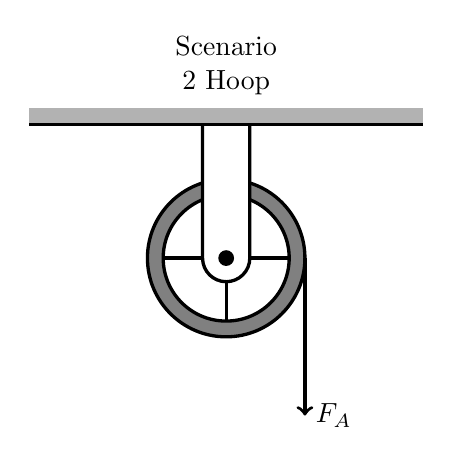
\begin{tikzpicture}[very thick]
          \draw[fill=gray] circle (1);
          \draw[fill=white] circle (.8);
          \draw (-.8,0)--(.8,0);
          \draw (0,0)--(0,-.8);
          \draw[->] (1,0)--+(0,-2) node[right]{$F_A$};
          \draw[fill=white] (-.3,1.7)--(-.3,0) arc (-180:0:.3)--(.3,1.7);
          \fill circle (.1);
          \fill[gray!60] (-2.5,1.7) rectangle +(5,.2)
          node[
            midway,
            above=4,
            text width=.7in,
            align=center,black]{Scenario 2 Hoop};
          \draw(-2.5,1.7)--+(5,0);
        \end{tikzpicture}
      \end{center}
      Scenarios 1 and 2 show two different pulleys. In Scenario 1, the pulley
      is the same solid disk referenced in part (a). In Scenario 2 , the pulley
      is a hoop that has the same mass $M$ and radius $R$ as the disk. Each
      pulley has a lightweight string wrapped around it several turns and is
      mounted on a horizontal axle, as shown. Each pulley is free to rotate
      about its centre with negligible friction.

      \vspace{.15in}In both scenarios, the pulleys begin at rest. Then both
      strings are pulled with the same constant force $F_A$ for the same time
      interval $\Delta t$, causing the pulleys to rotate without the string
      slipping. After time interval $\Delta t$, the change in angular momentum
      of the disk is equal to the change in angular momentum of the hoop, but
      the change in rotational kinetic energy for the disk is greater than that
      of the hoop.
    }
    \part Consider scenarios 1 and 2 at the end of time interval $\Delta t$. In
    a clear, coherent paragraph-length response that may also contain equations
    and drawings, explain why the change in angular momentum of both pulleys is
    the same but the change in rotational kinetic energy is greater for the
    disk.
  \end{parts}
  \newpage
  
  \uplevel{
    \centering
    \begin{tikzpicture}[scale=.65,thick]
      \draw circle (1);
      \draw circle (2);
      \fill circle (.1);
      \draw[axes,rotate=-30] (0,0)--(1,0) node[pos=.4,below left]{$r_0$};
      \draw[axes,rotate=20] (0,0)--(0,2) node[pos=.75,right=0]{$2r_0$};
      \draw (-2,0)--(-2,-4);
      \draw (1,0)--(1,-4.3);
      \draw (-2.4,-4) rectangle +(.8,-1.5) node[midway]{$m_0$};
      \draw (.3,-4.3) rectangle +(1.4,-1.8) node[midway]{$1.5m_0$};
      \draw[rotate=30] (0,0)--(3,0)
      node[right,text width=.6in]{Axle at Centre of Pulleys};
    \end{tikzpicture}  
  }
  \question Two pulleys with different radii are attached to each other so that
  they rotate together about a horizontal axle through their common centre.
  There is negligible friction in the axle. Object 1 hangs from a light string
  wrapped around the larger pulley, while object 2 hangs from another light
  string wrapped around the smaller pulley, as shown in the figure above.
  
  $m_0$ is the mass of object 1.\\
  $1.5m_0$ is the mass of object 2.\\
  $r_0$ is the radius of the smaller pulley.\\
  $2r_0$ is the radius of the larger pulley.

  \begin{parts}
    \part At time $t=0$, the pulleys are released from rest and the objects
    begin to accelerate.

    \begin{subparts}
      \subpart Derive an expression for the magnitude of the net torque exerted
      on the objects-pulleys system about the axle after the pulleys are
      released. Express your answer in terms of $m_0$, $r_0$, and physical
      constants, as appropriate.
      \vspace{\stretch1}

      \subpart Object 1 accelerates downward after the pulleys are released.
      Briefly explain why.
      \vspace{\stretch1}
    \end{subparts}
    \newpage
    
    \part At a later time $t=t_C$, the string of object 1 is cut while the
    objects are still moving and the pulley is still rotating. Immediately
    after the string is cut, how do the directions of the angular velocity and
    angular acceleration of the pulley compare to each other?

    \vspace{.15in}
    \underline{\hspace{.3in}}Same direction\hspace{.3in}
    \underline{\hspace{.3in}}Opposite directions

    \vspace{.15in}Briefly explain your reasoning.
    \vspace{\stretch1}

    \part On the axes below, sketch a graph of the angular velocity $\omega$ of
    the system consisting of the two pulleys as a function of time $t$. Include
    the entire time interval shown. The pulleys are released at $t=0$, and the
    string is cut at $t=t_C$.
    \begin{center}
      \vspace{.2in}
      \begin{tikzpicture}[xscale=.8,yscale=.6]
        \draw[gray,dashed] (0,-5) grid (10,5);
        \draw[axes] (0,0)--(10.7,0) node[right]{$t$};
        \draw[axes] (0,-5)--(0,5.7) node[above]{$\omega$};
      \end{tikzpicture}
    \end{center}
    \vspace{\stretch1}
  \end{parts}
  \newpage

  \uplevel{
    \cpic{.57}{cylinder-rolling}
  }
  \question A uniform cylinder of mass $m_0$ is placed at the top of an incline
  of length $L_0$ and height $H_0$, as shown above, and released from rest. The
  cylinder rolls without slipping down the incline and then continues rolling
  along a horizontal surface.
  \begin{parts}
    \part On the grid below, sketch a graph that represents the total kinetic
    energy of the cylinder as a function of the distance travelled by the
    cylinder as it rolls down the incline and continues to roll across the
    horizontal surface.
    \begin{center}
      \begin{tikzpicture}[yscale=.8]
        \draw[axes] (0,0)--(11,0) node[pos=0,below left]{$O$}
        node[midway,below=12]{Distance Travelled};
        \draw[axes] (0,0)--(0,5) node[
          midway,above,rotate=90,
          text width=1.3in,
          align=center]{Total Kinetic\\Energy};
        \foreach \y in {1,...,4} \draw[gray,thick,dashed] (0,\y)--(10,\y);
        \draw[thick,dashed] (5,0)--(5,4) node[pos=0,below]{$L_0$};
        \draw[thick,dashed] (10,0)--(10,4) node[pos=0,below]{$2L_0$};
      \end{tikzpicture}
    \end{center}

    \uplevel{
      \cpic{.57}{block-sliding}
      The cylinder is again placed at the top of the incline. A block, also of
      mass $m_0$, is placed at the top of a separate rough incline of length
      $L_0$ and height $H_0$, as shown above. When the cylinder and block are
      released at the same instant, the cylinder begins to roll without
      slipping while the block begins to accelerate uniformly. The cylinder and
      the block reach the bottoms of their respective inclines with the same
      translational speed.
    }
    \part In terms of energy, explain why the two objects reach the bottom of
    their respective inclines with the same translational speed. Provide your
    answer in a clear, coherent paragraph-length response that may also contain
    figures and/or equations.
  \end{parts}
\end{questions}
\end{document}
